\documentclass[12pt]{article}%

\usepackage{amsmath}
\usepackage{graphicx}
%Tambahan dari template

\begin{document}

\title{Machine Learning \protect\\ Assignment 1 \protect\\ CLO3} 
\author{Ida Bagus Dwi Satria Kusuma \protect\\ 1301140297}
\date{\today}
\maketitle

\begin{enumerate}
	\item In this problem we will consider similarity measures for movies on the Movielens dataset.
Download the Movielens data that we sent to you through email. In addition to the data, the file also contains some functions for easily loading the data into Matlab/Octave/R and some example code that you can use if you wish. See the README files for details.
	\begin{enumerate}	
		\item We will now construct a similarity measure over the movies. For simplicity, let us first consider a simple measure that does not use the explicit (numerical) ratings given by the users, nor the time stamps of the ratings, but only whether or not a given movie was rated by a given user. 
		\begin{enumerate}
			\item \textbf{(20 points)} Create a function that, given two different movie IDs as input, outputs the Jaccard coeffcient: the number of users who rated both movies divided by the number of users who rated at least one of the movies. For example, for the movies 'Toy Story' and 'GoldenEye' the coefficient should be 0.217.

			\par \textbf{Answer} Gunakan jaccard\_coeff.m untuk mendapatkan Jaccard Coefficient. Parameternya adalah dua id film yang ingin diukur.
			\par 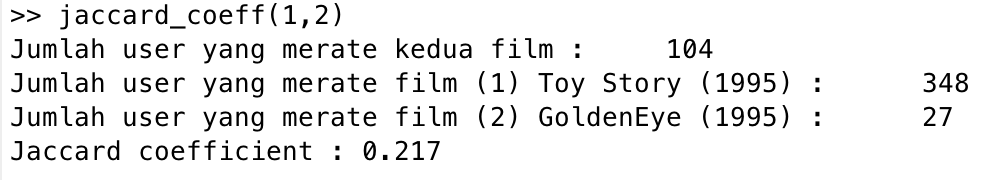
\includegraphics[width=10cm]{ss_13ai}
			% \begin{figure}[h]
				
			% \end{figure}

			\item \textbf{(5 points)} What is the Jaccard coefficient between 'Three Colors: Red' and 'Three Colors: Blue'?

			\par \textbf{Answer} Use searchMovie.m to get the movie's id and use jaccard\_coeff.m to get the Jaccard Coefficient.
			\par 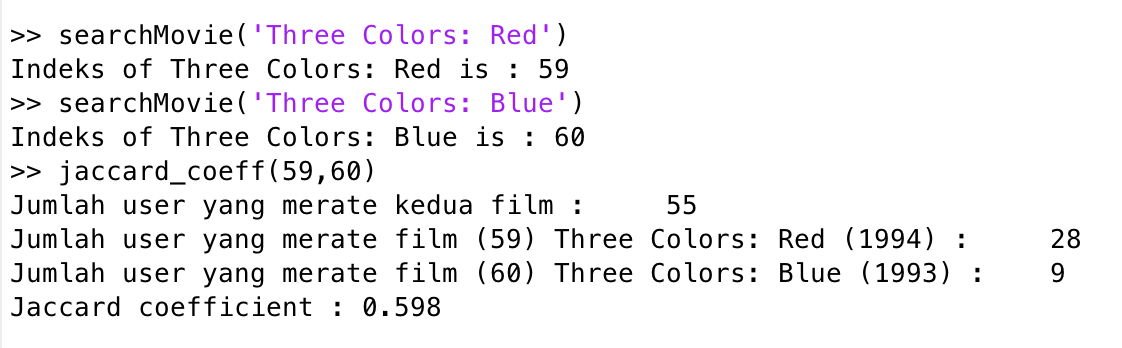
\includegraphics[width=10cm]{ss_13aii}

			\item \textbf{(10 points)} What are the 5 movies with highest Jaccard coefficient to 'Taxi Driver'?
			\par \textbf{Answer} Gunakan searchMovie.m untuk mendapatkan id film 'Taxi Driver' dan gunakan jaccard\_coeff\_n.m untuk mendapatkan film-film dengan Jaccard Coefficient sebanyak n tertinggi. dalam kasus ini, n = 5.
			\par 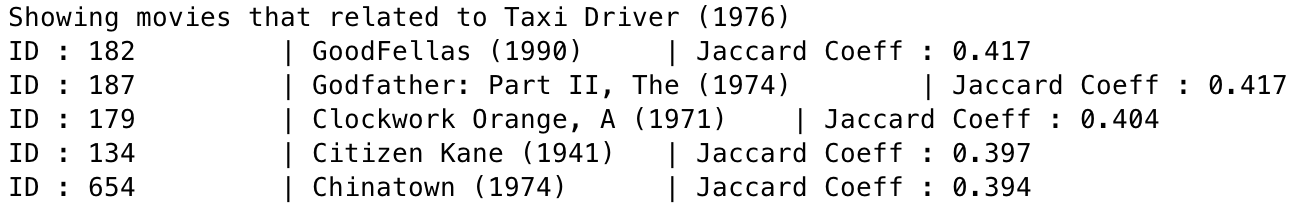
\includegraphics[width=10cm]{ss_13aiii}

			\item \textbf{(10 points)} Select a movie of your own choosing (which you are familiar with), what are the 5 movies with highest Jaccard coefficient to that movie? Do they make sense?

			\par \textbf{Answer} Gunakan searchMovie.m untuk mendapatkan id film 'Star Wars' dan gunakan jaccard\_coeff\_n.m untuk mendapatkan film-film dengan Jaccard Coefficient sebanyak n tertinggi. dalam kasus ini, n = 5.
			\par 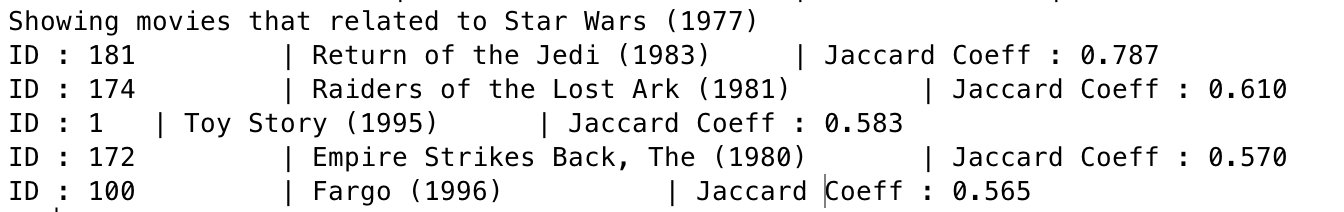
\includegraphics[width=10cm]{ss_13aiv}
		\end{enumerate}
	\end{enumerate}

\end{enumerate}
\end{document}

